\documentclass[11pt]{article}

\usepackage[margin=1in]{geometry}
\usepackage{setspace}
\onehalfspacing
\usepackage{graphicx}
\graphicspath{report_images/}
\usepackage{appendix}
\usepackage{listings}
\usepackage{float}
\usepackage{amsthm}

% DOCUMENT INFORMATION =================================================
\title {ECEN 429: Introduction to Digital Systems Design Laboratory \\ North Carolina Agricultural and Technical State University \\ Department of Electrical and Computer Engineering} % Declare Title
\author{Reporter: Nikiyah Beaulah\\ \and Partner: Chris Cannon} % Declare authors
\date{February 8, 2018}
% ======================================================================

\begin{document}

\maketitle % Render Title, Author, and Date

\begin{center}
Lab	2
\end{center}

\pagebreak

\section{Introduction}

\section{Background, Design Solution, and Results}

\subsection{Problem 1 Seven Segment Display}

\subsubsection{Background}
This problem prompted us to utilize the seven-segment display on the Basys3 board. Our input will be a 3-bit number so that we can provide input from 0-9, which is the range that can be displayed by a single seven-segment display. Seven-segment displays include, fittingly, seven segments. Those segments are conventionally referred to as a-g in accordance with Figure ~\ref{fig:sevenSegMap}.

\begin{figure}[h]
\begin{center}
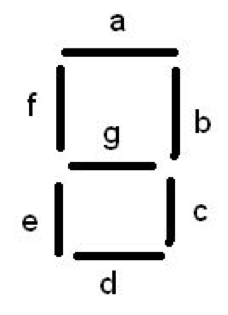
\includegraphics[width=0.2\textwidth]{report-images/img1.png}
\caption{Seven-Segment Display Map}
\label{fig:sevenSegMap}
\end{center}
\end{figure}

\subsubsection{Design Solution}
As discussed in the background for this problem, a seven-segment display can only display a single-digit 0-9. We have to use a 4-bit number in order to represent 9 (1001b) however, 10-15 (1010b-1111b) cannot be displayed using a single seven-segment display. In our code, this will be treated as an error condition where no data will be displayed on the seven-segment display. The 4-bit input will be x3 down to x0, with x3 as the most significant bit, and the output bits have been defined in the assignment. The input pin assignments are defined in Table ~\ref{tab:sevenSigInput} and the output pin assignments as well as their segment are defined in Table ~\ref{tab:sevenSigOutput}. The truth table for our seven segment decoder is shown in Table ~\ref{tab:sevenSegTruthTable}. During our design process, we remembered that the seven-segment display is "active-low", meaning that a '0' is treated as "ON" and a '1' is treated as "OFF". This was important when designing our truth table.

\begin{table}[h]
\begin{center}
	\begin{tabular}{| l | l | l |}
		\hline
		Bit & Label & Address \\ \hline
		x3 & Switch 3 & V17 \\ \hline
		x2 & Switch 2 & V16 \\ \hline
		x1 & Switch 1 & W16 \\ \hline
		x0 & Switch 0 & W15 \\ \hline
	\end{tabular}
	\caption{\label{tab:table-name}Input pin assignments for seven-segment decoder.}
	\label{tab:sevenSegInput}
\end{center}
\end{table}

\begin{table}[h]
\begin{center}
	\begin{tabular}{| l | l | l |}
		\hline
		Bit & Seven-Segment & Address \\ \hline
		out1 & a & W7 \\ \hline
		out2 & b & W6 \\ \hline
		out3 & c & U8 \\ \hline
		out4 & d & V8 \\ \hline
		out5 & e & U5 \\ \hline
		out6 & f & V5 \\ \hline
		out7 & g & U7 \\ \hline
	\end{tabular}
	\caption{\label{tab:table-name}Output pin assignments for seven-segment decoder.}
	\label{tab:sevenSegOutput}
\end{center}
\end{table}

\begin{table}[h]
\begin{center}
	\begin{tabular}{| l | l | l | l | l | l | l | l | l | l | l |}
		\hline
		x3 & x2 & x1 & x0  & out1 & out2 & out3 & out4 & out5 & out6 & out7\\ \hline
		0 & 0 & 0 & 0 & 0 & 0 & 0 & 0 & 0 & 0 & 1 \\ \hline
		0 & 0 & 0 & 1 & 1 & 0 & 0 & 1 & 1 & 1 & 1 \\ \hline
		0 & 0 & 1 & 0 & 0 & 0 & 1 & 0 & 0 & 1 & 0 \\ \hline
		0 & 0 & 1 & 1 & 0 & 0 & 0 & 0 & 1 & 1 & 0 \\ \hline
		0 & 1 & 0 & 0 & 1 & 0 & 0 & 1 & 1 & 0 & 0 \\ \hline
		0 & 1 & 0 & 1 & 0 & 0 & 1 & 0 & 0 & 1 & 0 \\ \hline
		0 & 1 & 1 & 0 & 0 & 1 & 0 & 0 & 0 & 0 & 0 \\ \hline
		0 & 1 & 1 & 1 & 0 & 0 & 0 & 1 & 1 & 1 & 1 \\ \hline
		1 & 0 & 0 & 0 & 0 & 0 & 0 & 0 & 0 & 0 & 0 \\ \hline
		1 & 0 & 0 & 1 & 0 & 0 & 0 & 0 & 1 & 0 & 0 \\ \hline
		1 & 0 & 1 & 0 & 1 & 1 & 1 & 1 & 1 & 1 & 1 \\ \hline
		1 & 0 & 1 & 1 & 1 & 1 & 1 & 1 & 1 & 1 & 1 \\ \hline
		1 & 1 & 0 & 0 & 1 & 1 & 1 & 1 & 1 & 1 & 1 \\ \hline
		1 & 1 & 0 & 1 & 1 & 1 & 1 & 1 & 1 & 1 & 1 \\ \hline
		1 & 1 & 1 & 0 & 1 & 1 & 1 & 1 & 1 & 1 & 1 \\ \hline
		1 & 1 & 1 & 1 & 1 & 1 & 1 & 1 & 1 & 1 & 1 \\ \hline
	\end{tabular}
	\caption{\label{tab:table-name}Truth table for seven-segment decoder.}
	\label{tab:sevenSegTruthTable}
\end{center}
\end{table}

\subsection{Results}

The resulting circuit successfully displayed the digit corresponding to each 4-bit number from 0-9. We were also able to correctly turn off all displays when an input greater than 9 was provided. Initially, the number 6 displayed incorrectly, we activated segment 'f' by mistake, therefore displaying '8'. Once this problem was identified, we were able to quickly address it and provide the correct output.

\begin{center}
	For the figures ~\ref{fig:sevenSegZero} through ~\ref{fig:sevenSegNine}, switches boxed in red are turned off and switches boxed in green are turned on.
\end{center}

\begin{figure}[H]
\begin{center}
\includegraphics[width=0.5\textwidth]{report-images/Part1/0.png}
\caption{Seven-Segment Display for "0000"}
\label{fig:sevenSegZero}
\end{center}
\end{figure}

\begin{figure}[H]
\begin{center}
\includegraphics[width=0.5\textwidth]{report-images/Part1/1.png}
\caption{Seven-Segment Display for "0001"}
\label{fig:sevenSegOne}
\end{center}
\end{figure}

\begin{figure}[H]
\begin{center}
\includegraphics[width=0.5\textwidth]{report-images/Part1/2.png}
\caption{Seven-Segment Display for "0010"}
\label{fig:sevenSegTwo}
\end{center}
\end{figure}

\begin{figure}[H]
\begin{center}
\includegraphics[width=0.5\textwidth]{report-images/Part1/3.png}
\caption{Seven-Segment Display for "0011"}
\label{fig:sevenSegThree}
\end{center}
\end{figure}

\begin{figure}[H]
\begin{center}
\includegraphics[width=0.5\textwidth]{report-images/Part1/4.png}
\caption{Seven-Segment Display for "0100"}
\label{fig:sevenSegFour}
\end{center}
\end{figure}

\begin{figure}[H]
\begin{center}
\includegraphics[width=0.5\textwidth]{report-images/Part1/5.png}
\caption{Seven-Segment Display for "0101"}
\label{fig:sevenSegFive}
\end{center}
\end{figure}

\begin{figure}[H]
\begin{center}
\includegraphics[width=0.5\textwidth]{report-images/Part1/6.png}
\caption{Seven-Segment Display for "0110"}
\label{fig:sevenSegSix}
\end{center}
\end{figure}

\begin{figure}[H]
\begin{center}
\includegraphics[width=0.5\textwidth]{report-images/Part1/7.png}
\caption{Seven-Segment Display for "0111"}
\label{fig:sevenSegSeven}
\end{center}
\end{figure}

\begin{figure}[H]
\begin{center}
\includegraphics[width=0.5\textwidth]{report-images/Part1/8.png}
\caption{Seven-Segment Display for "0100"}
\label{fig:sevenSegEight}
\end{center}
\end{figure}

\begin{figure}[H]
\begin{center}
\includegraphics[width=0.5\textwidth]{report-images/Part1/9.png}
\caption{\label{fig: fig-name} Seven-Segment Display for "1001"}
\label{fig:sevenSegNine}
\end{center}
\end{figure}

\pagebreak

\subsection{Problem 2 1:2 Decoder}

\subsubsection{Background}
The task posed for this problem was to develop a 1:2 decoder and implement it on the Basys3. The design will include 2 inputs, a 1-bit number and an enable bit.

\subsubsection{Design Solution}
The 1:2 decoder will accept a 1-bit input 'a', and is controlled by the bit 'sel'. The output is made up of bits 'out1' and 'out2'. The ports are described in Table ~\ref{tab:decoderPort}.

\begin{table}[h]
\begin{center}
		\begin{tabular}{| l | l | l |}
			\hline
			Bit & Label & Address \\ \hline
			a & Switch 0 & V17 \\ \hline
			sel & Switch 1 & V16 \\ \hline
			out1 & LED 0 & U16 \\ \hline
			out2 & LED 1 & E19 \\ \hline
		\end{tabular}
		\caption{\label{tab: tab-name} Input and output port assignments for 1:2 decoder.}
		\label{tab:decoderPort}
\end{center}
\end{table}

The decoder will only produce input when 'sel', the enable bit, is HIGH. When 'sel' is HIGH, the decoder will activate the 'out1' bit, representing the decimal value "0". When 'a' is HIGH when 'sel' is HIGH, the decoder will activate the 'out2' bit, representing the decimal value "1". This is summarized in Table ~\ref{tab:decoderTruthTable}.

\begin{table}[h]
\begin{center}
	\begin{tabular}{| l | l | l | l |}
		\hline
		a & sel & out1 & out2 \\ \hline
		0 & 0 & 0 & 0 \\ \hline
		0 & 1 & 1 & 0 \\ \hline
		1 & 0 & 0 & 0 \\ \hline
		1 & 1 & 0 & 1 \\ \hline
	\end{tabular}
	\caption{\label{tab:decoderTruthTable} Truth table for 1:2 decoder.}
	\label{tab:decoderTruthTable}
\end{center}
\end{table}

\subsubsection{Results}

\subsection{Problem 3 SUM of a Full Adder}

\subsubsection{Background}

A full adder is designed to incorporate both a carry-in and carry-out bit, which makes it more modular and allows us to build multi-bit adders. For this problem, we are to design a full adder that will accept a carry-in, a carry-out, and perform addition of two bits.

\theoremstyle{definition}
\newtheorem{definition}{Definition}
\begin{definition}
Carry-in Bit: the carry-in bit represents a 1-bit overflow from a previous addition operation. Because a full adder is intended to be modular, and build adders of multiple bits, it is important that the previous operation be available. For purposes of this lab, the carry-in for a 1 bit adder will be tied to ground.
\end{definition}

\begin{definition}
	Carry-out Bit: the carry-out bit represents a 1-bit overflow from the current addition operation. This can either be used to signal an error condition or to tie this adder in with multiple full adders. The result of this addition operation will either between 0 and 3. If the output is 2 or 3, the carry-out bit will be HIGH to signal that there is an additional bit needed to represent the results of this operation.
\end{definition}

\subsubsection{Design Solution}

For our solution, the two 1-bit inputs are designated as 'A' and 'B'. Carry-in is denoted as 'CI' and carry-out is denoted as 'CO'. The output sum of the adder will be represented by 'SUM'. The truth table for a full adder is represented in Table ~\ref{tab:fullAddTruthTable}.

\begin{table}[h]
\begin{center}
	\begin{tabular}{| l | l | l | l | l |}
		\hline
		A & B & CI & SUM & CO \\ \hline
		0 & 0 & 0 & 0 & 0 \\ \hline
		0 & 0 & 1 & 1 & 0 \\ \hline
		0 & 1 & 0 & 1 & 0 \\ \hline
		0 & 1 & 1 & 0 & 1 \\ \hline
		1 & 0 & 0 & 1 & 0 \\ \hline
		1 & 0 & 1 & 0 & 1 \\ \hline
		1 & 1 & 0 & 0 & 1 \\ \hline
		1 & 1 & 1 & 1 & 1 \\ \hline
	\end{tabular}
	\caption{\label{tab:fullAddTruthTable}Truth table for a full adder.}
	\label{tab:fullAddTruthTable}
\end{center}
\end{table}

Our full bit adder uses switches as all inputs and LEDs as outputs. The port assignment for the inputs and outputs is specified in Table ~\ref{tab:fullAddPorts}.

\begin{table}[h]
\begin{center}
	\begin{tabular}{| l | l | l |}
		\hline
		Bit & Label & Port \\ \hline
		A & Switch 0 & V17 \\ \hline
		B & Switch 1 & V16 \\ \hline
		CI & Switch 2 & W16 \\ \hline
		CO & LED 1 & E19 \\ \hline
		SUM & LED 0 & U16 \\ \hline
	\end{tabular}
	\caption{\label{tab:fullAddPorts}Port assignment for full adder.}
	\label{tab:fullAddPorts}
\end{center}	
\end{table}

\subsubsection{Results}

\section{Conclusion}

\end{document}
